\documentclass[tikz,border=2pt]{standalone}
\usepackage{amsmath,amssymb}
\usetikzlibrary{arrows.meta}
\begin{document}
% EPQ optimum for d = 2, r = 8, K = 100, h = 1, b = 3: s* = -5, S* = 15, g* = 15.
% Machine off: level falls at rate d = 2 for t_1 = 10 days; machine on: rises at r - d = 6
% for t_2 = 10/3 days; cycle T = 40/3. Positive part (holding) blue, backlog red.
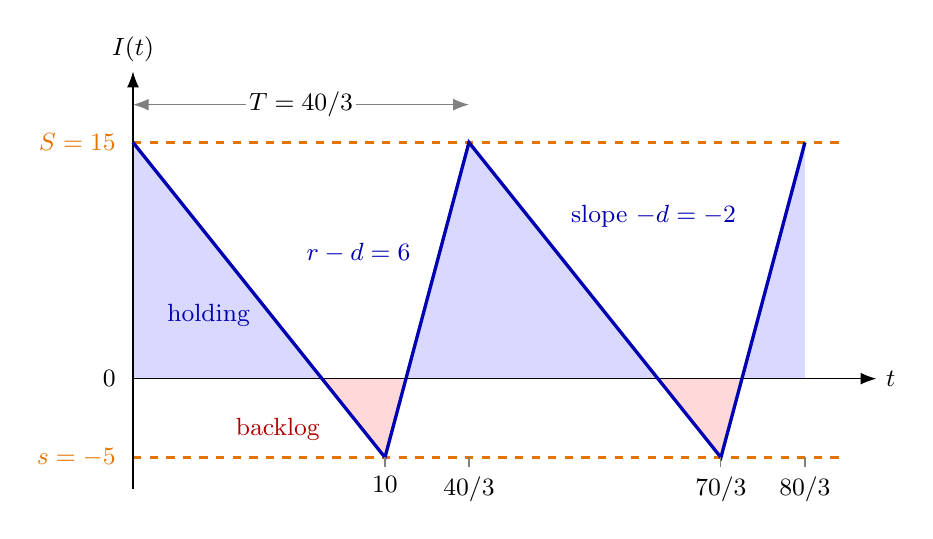
\begin{tikzpicture}[font=\small, >={Latex[length=2mm]}, x=0.32cm, y=0.2cm]
  % triangles
  \fill[blue!15] (0,0) -- (0,15) -- (7.5,0) -- cycle;
  \fill[blue!15] (10.833,0) -- (13.333,15) -- (20.833,0) -- cycle;
  \fill[blue!15] (24.167,0) -- (26.667,15) -- (26.667,0) -- cycle;
  \fill[red!15] (7.5,0) -- (10,-5) -- (10.833,0) -- cycle;
  \fill[red!15] (20.833,0) -- (23.333,-5) -- (24.167,0) -- cycle;
  % policy levels
  \draw[orange!90!black, thick, dashed] (0,15) -- (28,15);
  \draw[orange!90!black, thick, dashed] (0,-5) -- (28,-5);
  \node[orange!90!black, anchor=east] at (-0.3,15) {$S=15$};
  \node[orange!90!black, anchor=east] at (-0.3,-5) {$s=-5$};
  % axes
  \draw[->] (0,0) -- (29.5,0) node[right] {$t$};
  \draw[->] (0,-7) -- (0,19.5) node[above] {$I(t)$};
  \node[anchor=east] at (-0.3,0) {$0$};
  % inventory level
  \draw[blue!70!black, very thick] (0,15) -- (10,-5) -- (13.333,15) -- (23.333,-5) -- (26.667,15);
  % epochs
  \foreach \x/\l in {10/10, 13.333/{40/3}, 23.333/{70/3}, 26.667/{80/3}}
    {\draw[gray] (\x,-5) -- (\x,-5.6) node[below, black] {$\l$};}
  % slopes
  \node[blue!70!black, anchor=south west] at (17,9) {slope $-d=-2$};
  \node[blue!70!black, anchor=east] at (11.4,8) {$r-d=6$};
  % cycle length
  \draw[<->, gray] (0,17.4) -- (13.333,17.4) node[midway, fill=white, inner sep=1pt, text=black] {$T=40/3$};
  % cost labels
  \node[blue!70!black] at (3.0,4.0) {holding};
  \node[red!70!black, anchor=east] at (7.8,-3.2) {backlog};
\end{tikzpicture}
\end{document}
